\documentclass[12pt]{article}

\usepackage[magyar]{babel}
\usepackage{t1enc}
\usepackage{times}
% \usepackage{lipsum}
\usepackage{graphicx}
\graphicspath{ {./} }
\usepackage[]{hyperref}
\hypersetup{
    colorlinks=true,
    linkcolor=blue,
    filecolor=magenta,
    urlcolor=cyan
}
\usepackage[backend=biber]{biblatex}
% \usepackage[]{biblatex}
\addbibresource{hivatkozasok.bib}

\usepackage{listings}

\usepackage{xcolor}

\definecolor{codegreen}{rgb}{0,0.6,0}
\definecolor{codegray}{rgb}{0.5,0.5,0.5}
\definecolor{codepurple}{rgb}{0.58,0,0.82}
\definecolor{backcolour}{rgb}{0.95,0.95,0.92}

\lstdefinestyle{mystyle}{
    backgroundcolor=\color{backcolour},
    commentstyle=\color{codegreen},
    keywordstyle=\color{magenta},
    numberstyle=\tiny\color{codegray},
    stringstyle=\color{codepurple},
    basicstyle=\ttfamily\footnotesize,
    breakatwhitespace=false,
    breaklines=true,
    captionpos=b,
    keepspaces=true,
    numbers=left,
    numbersep=5pt,
    showspaces=false,
    showstringspaces=false,
    showtabs=false,
    tabsize=2
}

\lstset{style=mystyle}

%A fejléc láblécek kialakításához:
\usepackage{fancyhdr}

%Margók:
\hoffset -1in
\voffset -1in
\oddsidemargin 35mm
\textwidth 150mm
\topmargin 15mm
\headheight 10mm
\headsep 5mm
\textheight 237mm

\author{Südi Tamás}
\title{Terhelés-kiegyenlítés AP-asszisztált roaming segítségével OpenWrt-en}
\makeatletter

\begin{document}

%A FEJEZETEK KEZDŐOLDALAINAK FEJ ES LÁBLÉCE:
%a plain oldalstílust kell átdefiniálni, hogy ott ne legyen fejléc:
\fancypagestyle{plain}{%
%ez mindent töröl:
\fancyhf{}
% a láblécbe jobboldalra kerüljön az oldalszám:
\fancyfoot[R]{\thepage}
%elválasztó vonal sem kell:
\renewcommand{\headrulewidth}{0pt}
}

%A TÖBBI OLDAL FEJ ÉS LÁBLÉCE:
\pagestyle{fancy}
\fancyhf{}
\fancyhead[L]{\@title}
\fancyfoot[R]{\thepage}


%A címoldalra se fej- se lábléc nem kell:
\thispagestyle{empty}

\begin{center}
\vspace*{1cm}
{\Large\bf Szegedi Tudományegyetem}

\vspace{0.5cm}

{\Large\bf Informatikai Intézet}

\vspace*{3.8cm}


{\LARGE\bf \@title}


\vspace*{3.6cm}

{\Large Szakdolgozat}

\vspace*{4cm}

{\begin{center}
  \begin{tabular}{ccc}
  \emph{Készítette:} & \emph{Külső témavezető:} & \emph{Belső témavezető:}\\
  \bf{Südi\ Tamás} & \bf{Dr.\ Kelemen András} & \bf{Csirik\ János}\\
  programtervező informatikus & egyetemi docens & egyetemi tanár\\
  szakos hallgató
  \end{tabular}
\end{center}}

\vspace*{2.3cm}

{\Large
Szeged
\\
\vspace{2mm}
\the\year{}
}
\end{center}


%A tartalomjegyzék:
\tableofcontents

\section*{Feladatkiírás}


A témavezető által megfogalmazott feladatkiírás. Önálló oldalon szerepel.
\newpage

\section*{Tartalmi összefoglaló}

% A tartalmi összefoglalónak tartalmaznia kell (rövid, legfeljebb egy oldalas, összefüggő megfogalmazásban)
% a következőket: a téma megnevezése, a megadott feladat megfogalmazása - a feladatkiíráshoz viszonyítva-,
%a megoldási mód, az alkalmazott eszközök, módszerek, az elért eredmények, kulcsszavak (4-6 darab).
%
%Az összefoglaló nyelvének meg kell egyeznie a dolgozat nyelvével. Ha a dolgozat idegen nyelven készül,
%magyar nyelvű tartalmi összefoglaló készítése is kötelező (külön lapon), melynek terjedelmét a TVSZ szabályozza.

A dolgozat célja a centralizált AP-asszisztált roaming megvalósítása OpenWrt alapú rendszerekre.
A dolgozat célja továbbra, hogy bemutassa az OpenWrt rendszert, a roaming technikákat és a szükséges 802.11 protokollokat.

A dolgozat első fejezete az OpenWrt rendszer bemutatásával és telepítésével foglalkozik. Összehasonlítja a virtuális fejlesztői környezet előnyeit és hátrányait a fizikai környezettel, telepítés, használat, sebesség és konfigurálhatóság szempontjából.
A dolgozat második fejezete a hálózati protokollokkal, a roaming technikákkal és a szükséges 802.11 protokollok bemutatásával foglalkozik, ismerteti az AP-asszisztált roamingot.
A dolgozat harmadik fejezete a terhelés-kiegyenlítési algoritmusokkal foglalkozik.
A dolgozat negyedik részében az éles környezetben történő tesztelésről és a kapott eredményekről szól.
A dolgozat utolsó fejezete a szakirodalmat és a kapcsolódó projekteket mutatja be.

\newpage

\section{Az OpenWrt rendszer bemutatása}

Az OpenWrt egy Linux-alapú, nyílt forráskódú, hálózati eszközökhöz készült operációs rendszer.

Az OpenWrt a gyártói firmware helyett telepíthető a támogatott eszközökön. Ahhoz képest számos előnyt kínál a felhasználóknak, beleértve a letisztultságot, a nagyobb testreszabhatóságot, több funckiót és jobb biztonságot.

A legtöbb komponens és a build rendszer a GNU General Public License Version 2 licensz alatt érhető el, azonban néhány, elsősorban a nem OpenWrt-ben létrehozott részek más licensek alatt állnak. \cite{openwrt_about} \cite{openwrt_faq} \cite{openwrt_home}

\subsection{Telepítés fizikai eszközre}

Egyes eszközök már rendelkeznek OpenWrt vagy OpenWrt alapú firmwarrel, azonban legtöbbször ennek telepítése a felhasználó feladata.

A támogatott eszközök listája a \url{https://openwrt.org/toh/start} oldalon található. Itt az eszköz támogatottságától és népszerűségétől függően megtalálhatóak annak specifikációi, a hozzá tartozó firmwarek letöltési linkje és a telepítési, visszaállítási útmútatók.

A telepítés folyamata eszközönként eltérő lehet, de általában az alábbi módokon történhet: az eszköz webes kezelőfelületen keresztül, FTP-n keresztül, SD-kártya vagy USB-meghajtó segítségével, soros port használatával. Ez azonban a garancia elvesztésével és az eszköz meghibásodásával járhat.

\cite{openwrt_install}
\cite{openwrt_stock}

\subsubsection{Telepítés ASUS TUF AX4200 eszközre}

Az én általam használt ASUS TUF AX4200 eszközre az alaplapon található soros porton keresztül telepítettem az OpenWrt-t. A telepítést el lehet végezni egy Raspberry PI segítségével is, de nekem rendelkezésemre állt egy USB-soros port átalakító, így azt használtam. \cite{asus_ax4200}

Az eszköz szétbontása rendkívül egyszerű, a lábakban található négy csavar eltávolítása után az előlap könnyedén lepattintható.

Az alaplapon egy négy csatlakozós sorosport található. A jelölés alapján a legfelső a táp, a második a földelés, a harmadik a TX, a negyedik pedig az RX. Mivel az eszköz rendelkezik saját táppal, ezért azt nem csatlakoztattam.

Mivel az eszközön fejlesztést és tesztelést tervezek végezni, így proaktivitás céljából a soros portra egy 3 pin-es csatlakozót forrasztottam, hogy a későbbiekben gyorsabban tudjam csatlakoztatni a számítógéphez.

\includegraphics*[scale=0.30]{./soros-port.jpg}

\begin{lstlisting}
  Please choose the operation:
    1: Load System code to SDRAM via TFTP.
    2: Load System code then write to Flash via TFTP.
    3: Boot System code via Flash (default).
    4: Entr boot command line interface.
    7: Load Boot Loader code then write to Flash via Serial.
    9: Load Boot Loader code then write to Flash via TFTP.
\end{lstlisting}


Ezután elindítottam az eszközt és a 4-es gomb nyomva tartásával megszakítottam a boot folyamatot és beléptem egy CLI-be.

Eztán az eszköz LAN1 portját egy Ethernet kábellel a számítógépemhez csatlakoztattam és a számítógépem hálózatát statikusra állítottam, hogy felvegyem a 192.168.1.66 címet és a /24-es maszkot.

A routeren az alábbi parancsok megadásával elindítottam a lecsúpasított OpenWrt rendszert:

\begin{lstlisting}[language=bash]
  setenv ipaddr 192.168.1.1
  setenv serverip 192.168.1.66
  tftpboot 0x46000000 openwrt.bin
  bootm 0x46000000
\end{lstlisting}

Ez az OpenWrt fájl nem tartalmazza a webes kezelőfelületet, ezért scp parancs segítségével húztam át a teljes firmwaret a routerre.

\begin{lstlisting}[language=bash]
  scp sudta@192.168.1.66:/tmp/openwrt-mediatek-filogic-asus_tuf-ax4200-squashfs-sysupgrade.bin /tmp
  sysupgrade -n /tmp/openwrt-mediatek-filogic-asus_tuf-ax4200-squashfs-sysupgrade.bin
\end{lstlisting}




\subsection{Telepítés virtuális környezetbe}

A virtuális környezet egy olyan szoftveres megoldás, ami lehetővé teszi azt, hogy a felhasználó egyszerre futtasson több, akár különböző operációs rendszert is a számítógépén.

A virtuális környezet rengeteg előnnyel járhat egy fejlesztő számára, mint például az extra eszköz használatának elkerülése, az egyszerűbb fájlátvitel, a kijelző és a billentyűzet használata, a gyorsabb hardver, mentések készítése és visszaállítása és ezek megosztása más fejlesztőkkel. Azonban az ilyen környezeteknek is lehetnek hátrányai, mint például, hogy a hálózati kártya nem rendelkezik a szükséges hardveres támogatással és nem olyan megbízható a teljesítménye, mint egy erre tervezett eszköznek.

\subsubsection{Virtuális környezet Linux alatt}

A Linux-alapú operációs rendszerek népszerűek a fejlesztők körében, mivel ingyenesek és számos olyan funkcióval rendelkeznek, amelyek lehetővé teszik a hatékony és kényelmes munkavégzést.

Ezen a platformon több virtuális környezet is elérhető, mint például a VirtualBox, a VMware Workstation vagy a KVM.

A nyílt forráskódú Kernel-based Virtual Machine (KVM) egyik előnye, hogy képes
átadni PCI csatlakozású eszközöket is virtuális gépnek, így alacsony szintű hozzáférést biztosít a hardverhez. \cite{kvm} \cite{pci_passthrough}

Több virtuális környezet kezelő alkalmazás is támogatja mind az USB, mind a PCI csatlakozású eszközök átadását. Én ezek közül a virt-manager nevű programot választottam.


Hogy egyszerűsítsem a telepítési folyamatot \href{https://github.com/uwzis/gpu-passthrough-manager}{gpu-passthrough-manager} nevű szoftvert használtam, amely segítségével felkészítettem a rendszeremet a PCI csatornán keresztül csatlakozó WLAN-vezérlő átadására.

% kernelparaméterrel indítsa el. Ez hülyén hangzik
Ezután már csak meg kellett adnom a grub rendszerbetöltőnek, hogy a rendszert a vfio-pci.ids=8086:06f0 kernelparaméterrel indítsa el, amely a laptopom WLAN-vezérlő azonosítóját jelöli.

% Ehhez ugye nem kell forrást megjelölnöm?

A számítógépem architektúrájának megfelelően a \href{https://downloads.openwrt.org/releases/22.03.2/targets/x86/64/openwrt-22.03.2-x86-64-generic-ext4-combined.img.gz}{openwrt-22.03.2-x86-64-generic-ext4-combined.img} képet használtam a virtuális gép létrehozásához. Ez nem tartalmaz semmilyen telepítőt, helyette grub rendszerbetöltő segítségével indítja el a rendszert.

\subsubsection{Virtuális környezet Windows alatt Hyper-V segítségével}

A Hyper-V a Microsoft Windows natív virtualizációs környezete.

Ezt használja például a fejlesztők által kedvelt Windows Subsystem for Linux (WSL) Version 2 is, amely lehetővé teszi a Linux kernel futtatását Windows alatt, így alacsonyabb szintű hozzáférést biztosít a hardverhez. \cite{wsl2} \cite{hyperv_pci} Bár a Hyper-V képes bizonyos eszközök átadására a virtuális gépnek, de ezeket a funkciókat a WSL2 nem támogatja.

A Hyper-V eszközátadás protokolljának fejlesztésekor a cél eszközök nem hálózati kontrollerek, hanem perifériák és tárolóeszközök voltak. \cite{wsl2_usbip}

\subsubsection{Virtuális környezet Oracle VirtualBox segítségével}

Az Oracle VirtualBox egy multiplatform virtuális környezet, amely használatához először le kell tiltani a Hyper-V-t Windows alapú rendszereken. \cite{virtualbox_and_hyperv}
Ezt legegyszerűbben a host rendszeren futó parancssorból lehet elvégezni:

\begin{lstlisting}[language=Bash]
  bcdedit /set hypervisorlaunchtype off
\end{lstlisting}

Habár az Oracle Virtualbox nem támogatja a .img kiterjesztésű képeket, de tartalmazza a VBoxManage nevű programot, amely segítségével az img kép átkonvertálható .vdi kiterjesztésű virtuális lemezzé.

\begin{lstlisting}[language=Bash]
  & 'C:\Progra~1\Oracle\VirtualBox\VBoxManage.exe' convertfromraw  --format VDI '.\openwrt-22.03.3-x86-64-generic-ext4-combined.img' '.\openwrt.vdi'
\end{lstlisting}

Az újonnan létrejött openwrt.vdi kép segítségével létrehozható a virtuális gép. Alapértelmezetten a host gépről nem érhető el a virtuális gép hálózata, azonban ez megoldható port-forwarding szabályok felvétele segítségével a Virtuális gép beállításainak Hálózat / adapter1 / speciális / port forwarding menüpontjában.

\newpage

\subsection{Hálózat beállítása OpenWrt rendszeren}

\subsection{A WAN port beállítása}

A Wide Area Network (WAN) port a routert egy másik hálózathoz csatlakoztatja, amely lehet egy másik router, de akár közvetlenül az internet is.

Az OpenWrt indítása után lehetséges, hogy az internethez való csatlakozás nem sikerül. Ennek ellenőrzését a ping parancs segítségével lehet elvégezni:

\begin{lstlisting}[language=Bash]
  root@OpenWrt:/# ping vanenet.hu
  ping: bad address 'vanenet.hu'
  root@OpenWrt:/# ping 1.1.1.1
  PING 1.1.1.1 (1.1.1.1): 56 data bytes
  ping: sendto: Network unreachable
\end{lstlisting}

Ha a ping parancs nem sikerül, akkor valószínűleg a WAN porthoz tartozó interface konfigurációja nem megfelelő. Ezt a /etc/config/network fájlban lehet szerkeszteni.

Ha a csatlakozó hálózaton DHCP szerver üzemel, akkor az alábbi módosításokkal lehet a DHCP protokollt engedélyezni:

\begin{lstlisting}[]
  config interface 'lan'
       option device 'br-lan'
  +    option proto 'dhcp'
  -    option proto 'static'
  -    option ipaddr '192.168.1.1'
  -    option netmask '255.255.255.0'
  -    option i6assign '60'
\end{lstlisting}

A változtatások érvényesítéséhez újra kell indítani a network szolgáltatást.

Ezt a következő parancs segítségével lehet elvégezni:

\begin{lstlisting}[language=Bash]
   service network restart
\end{lstlisting}

Ezután a ping parancs segítségével lehet ellenőrizni, hogy a WAN port beállítása sikeres volt-e:

\begin{lstlisting}[language=Bash]
  root@OpenWrt:/# ping vanenet.hu
  PING vanenet.hu (185.33.54.12): 56 data bytes
  64 bytes from 185.33.54.12: seq=0 ttl=54 time=8.351 ms
  64 bytes from 185.33.64.12: seq=1 ttl=54 time=8.104 ms
  64 bytes from 185.33.64.12: seq=2 ttl=54 time=7.570 ms
\end{lstlisting}


\subsection{A WLAN beállítása}

Az eszközhöz készített image általában tartalmazza a szükséges drivereket, ekkor a WLAN beállítása egyszerűen megoldható a webes felületen keresztül.

Lehetséges azonban, hogy ezeket manuálisan kell telepíteni. Az \texttt{opkg} csomagkezelő segítségével lehet beszerezni a szükséges csomagokat. A telepítéshez először frissíteni kell a csomaglistát:

\begin{lstlisting}[language=Bash]
  root@OpenWrt:/# opkg update
\end{lstlisting}

Ez a parancs letölti az internetről a RAM-ba a csomaglistát, majd a \texttt{list} parancs segítségével megtekinthető a letöltött csomagok listája.

Ezután a gyártóhoz tartozó kernel modult is telepíteni kell. Intel eszközök esetében ezt a \texttt{kmod-iwlwifi} csomag biztosítja. A telepítés után engedélyezni kell a modult, majd újra kell indítani a rendszert. \cite{iwlwifi}

\begin{lstlisting}[language=Bash]
  root@OpenWrt:/# opkg install kmod-iwlwifi
  root@OpenWrt:/# modprobe iwlwifi
  root@OpenWrt:/# reboot
\end{lstlisting}

Ha ezután sem jelenik meg a WLAN interface, akkor valószínűleg nincsen telepítve a szükséges meghajtó. A \texttt{dmesg} parancs segítségével lehet megtekinteni a rendszerüzeneteket, és ebből kideríteni, hogy melyik drivert kell telepíteni.

\begin{lstlisting}
  [ 4.953303] iwlwifi 0000:07:00.0: Direct firmware load for iwlwifi-QuZ-a0-hr-b0-39.ucode failed with error -2
  [ 4.957677] iwlwifi 0000:07:00.0: minimum version required: iwlwifi-QuZ-a0-hr-b0-39
  [ 4.958681] iwlwifi 0000:07:00.0: maximum version supported: iwlwifi-QuZ-a0-hr-b0-66
\end{lstlisting}

A fenti üzenet azt jelenti, hogy a \texttt{iwlwifi-QuZ-a0-hr-b0-xx.ucode} fájl hiányzik, és ezt kell telepíteni. A népszerűbb driverek elérhetőek az OPKG csomagkezelőben, de gyártói oldalakról is letölthetőek.
Az Ubuntu operációs rendszer készítői egy olyan tárolót tartanak fent, ami tartalmazza a legtöbb gyártóhoz tartozó illesztőprogramokat.

Ezt az alábbi linken lehet elérni: \href[]{https://git.launchpad.net/~ubuntu-kernel/ubuntu/+source/linux-firmware/tree/}{https://git.launchpad.net/~ubuntu-kernel/ubuntu/+source/linux-firmware/tree/}

Innen az OpenWrt eszköz \texttt{/lib/firmware/} könyvtárába kell másolni a megfelelő fájlt. A fenti példában ez a \texttt{iwlwifi-QuZ-a0-hr-b0-66.ucode} fájl lenne.
% TODO: move files to /lib/firmware


\section{Vezeték nélküli hálózati protokollok és fogalmak}
\subsection{Az IEEE 802.11 Wi-Fi szabványcsalád}

Az Institute of Electrical and Electronics Engineers
(IEEE) nemzetközi szakmai szervezet 802 szabványcsaládja definiálja a legismertebb vezeték hálózati szabványokat.
Ennek a kollekciónak a része a 802.11 Wi-Fi család is, amely a lokális vezeték nélküli mikrohullám alapú kommunikációt szabványosítja.

Az osztályban a legismertebb szabványok az a, b, g, n, ac, ax 802.11 protokollok.
 A szabványok közötti különbség a frekvenciasávban, a jelerősségben, a csatornaszélességben, a modulációs technikában és ezáltal a maximális adatátviteli sebességben rejlik.

 \subsection{Wi-Fi Access Point}

Az Wi-Fi Access Point egy olyan hálózati eszköz, amely lehetővé teszi a vezeték nélküli csatlakozást a hálózathoz.

\subsection{Wi-Fi Station}

A "Wi-Fi állomás" (STA) egy olyan általános kifejezés, amely egy olyan eszközt jelent, amely csatlakozik egy Wi-Fi hálózathoz. Ez lehet egy laptop, egy okostelefon, egy IoT eszköz vagy egy vezeték nélküli repeater is.


\subsection{SSID}

Az SSID (Service Set Identifier) egy karakterlánc típusú azonosító, amelyet a hálózat sugároz a környezetébe. Ez által a felhasználók könnyen azonosíthatják és megkülönböztethetik a hálózatokat egymástól.

\subsection{BSS}

A Basic Service Set (BSS) arra utal, hogy az adott objektum egy primitív építőeleme a szolgáltatásnak. Wi-Fi hálózatok esetében ez egyetlen hozzáférési pont, amelyet a BSSID-ja azonosít. Ez általában az adott eszköz MAC címe.

Fontos megjegyezni, hogy egy BSS több SSID-t is sugározhat és egy fizikai eszközbe több BSS is beépíthető. A 2.4 és 5 GHz-et is támogató \texttt{dual-band AP}-k általában két BSS-t is tartalmaznak.


\subsection{Frekvenciasávok és csatornák}

A legegyszerűbben Wi-Fi szabványok a 2,4 GHz és az 5 GHz elnevezésű frekvenciasávokat használják.

A 2,4 GHz-es sáv a régebbi és elterjedtebb frekvenciasáv, amely a 2400 és 2483 MHz közötti tartományba esik. Mivel ez a sáv szabadon használható, azt más eszközök, például mikrohullámú sütők, Bluetooth eszközök vagy rádiók is használhatják.

Az 5 GHz-es sáv csak az újabb Wi-Fi szabványok támogatják, mint például a 802.11ac és a 802.11ax. Ez a 5160 és 5895 MHz közötti szélesebb frekvenciasávot használja.
Ez nagyobb sávszélességeset és kevesebb interferenciát kínál, ezáltal jobb teljesítményt eredményez. Azonban terjedése gyengébb, ezért a társánál rövidebb hatótávolságot biztosít.

A Wi-Fi kontextusában a frekvenciasávok mellett beszélhetünk csatornákról is, amelyek az adott frekvenciasávokhoz rendelt azonosítók.

Az eszközök általában több szomszédos csatornát, azaz szélesebb frekvenciasávokat, például 20, 40, 80 vagy akár 160 MHz-et is felhasználhatnak, ha képesek erre a helyi szabályozások is engedélyezik ezt. \cite{wlan_channels}

Azonban annak ellenére, hogy egy eszköznek van tanúsítványa egy adott frekvenciasávhoz, nem feltétlenül tudja használni az összes csatornát abban.

\subsection{Átviteli sebesség}

Az átviteli sebesség azt jelenti, hogy adott időablakban milyen mennyiségű adatot képes átadni az eszköz a hálózaton.

Az elérhető sebességet általában az alábbi tulajdonságokkal írjuk le:

\subsubsection{Moduláció és kódolás}

A moduláció és kódolás (MCS) tábla a használható jelek tulajdonságait, például a frekvenciájukat, a fázisukat és az amplitúdójukat határozza meg.

Az eszközök számos MCS érték közül választhatnak, az eszközök támogatása, a jel erőssége és a kommunikáció minőssége függvényében. Ezeket a https://mcsindex.com/ oldalon lehet megtekinteni. Az alacsonyabb MCS értékek általában alacsonyabb sebességet, míg a magasabb MCS értékek magasabb sebességet biztosítanak.

\subsubsection{Időosztás és más osztási technikák}

Az időosztás egy olyan technika, amely lehetővé teszi, hogy több eszköz egyidejűleg kommunikáljon az adott hálózaton.
Ilyenkor egy adott időintervallum felosztásra kerül
több szeletre, amelyekben a kliensek egymást váltva kommunikálhatnak.

A vezetéknélküli hálózatok más osztási technikákat is alkalmazhatnak.

A Code Division technika segítségével az eszközök különböző kódolások használatával egymástól függetlenül és egyidejűleg használják ugyanazt a frekvenciasávot. A kódok merőlegessége lehetővé teszi az adatok elkülönítését a fogadó oldalon.

A MIMO (Multiple-Input Multiple-Output) rendszerek segítségével az eszközök különböző irányokba mutató antennákat használnak, amelyek lehetővé teszik az adatok irányított átvitelét és fogadását. Ezáltal az eszközök egymástól függetlenül és egyidejűleg kommunikálhatnak ugyanazon a frekvenciasávon, minimalizálva az interferenciát és növelve a kapacitást.


\subsubsection{Interferencia}

Az interferencia a vezetéknélküli hálózatokban előforduló jelenség, amely akkor következik be, amikor egy adott jel egy másik jelre hatást gyakorol. Ekkor a zavaró jelet zajnak nevezzük.

Ennek eredményeképpen a jel torzul és az átvitel minősége romlik, azonban ez nem feltétlenül eredményez hibás adatokat, mivel a kódolási technikák ezt megakadályozzák ellenőrzés és javítás segítségével.

\subsubsection{A távolság hatása}

A távolság növekedésével a jel erőssége csökken, több zavaró jel kerül annak útjába és elnyelődhet vagy rosszabb esetben visszaverődhet, ezáltal zajt okozva.






\subsection{Authentikáció}

Az authentikáció a hálózatban történő az azonosítási folyamatot jelenti, amely során a felhasználó azonosítja magát a hálózat felé. Ez általában jelszóval vagy valamely egyéb közös kulcsú titkosítás (Shared Key) használatával történik.
Az authentikáció bekapcsolása erősen ajánlott, de nem kötelező.

\subsection{Asszociáció}

Az asszociáció a Wi-Fi hálózatokban a csatlakozási folyamatot jelenti, amely során az eszközök kapcsolatot létesítenek és azonosítják magukat a hálózaton belül. Amikor egy eszköz csatlakozni kíván egy Wi-Fi hálózathoz, asszociációs kérelemmelet küld ki. A hálózat válaszolva elfogadja vagy elutasítja az asszociációs kérést. Az asszociáció során az eszköz és a hálózat között kialakul egy kapcsolat, amely lehetővé teszi az adatátvitelt és a kommunikációt a hálózaton belül. Az asszociáció folyamata során a hálózat azonosítja és hitelesíti az eszközt, valamint hozzárendelhet egy azonosítót.
Ez lehetővé teszi az eszköz számára, hogy részt vegyen a hálózati kommunikációban és hozzáférjen a hálózat erőforrásaihoz.

\subsection{DHCP}

A DHCP (Dynamic Host Configuration Protocol) egy hálózati protokoll, amely nemcsak a vezeték nélküli hálózatokban, hanem általában az IP-alapú hálózatokban is használatos. Ez tájékoztatja a klienst a hálózat felépítéséről és a saját azonosítájáról.

Ez a folyamat egy három lépéses úgy nevezett "kézfogással" zajlik le.

Az első lépésben a kliens egy DHCP Discovery üzenetet szór szét a hálózaton, amelyben kéri a DHCP szervert, hogy válaszoljon neki.

Erre a DHCP szerver egy DHCP Offer üzenettel válaszol, amelyben megadja a kliens számára a hálózat konfigurációját.

A kliens a DHCP Request üzenetében visszaigazolja a DHCP szervernek, hogy elfogadja a konfigurációt, amely erre egy ACK üzenettel válaszol.


\subsection{Wi-Fi irányítási protokollok}

A Wi-Fi hálózatkezelési protokollok a hálózatok működését segítik. A hálózatok működéséhez szükséges az eszközök szabályozása is. Ezt a feladatot látják el a Wi-Fi irányítási protokollok. Nem minden hálózati eszköznek kell mindegyiket támogatnia, de ezek segíthetnek a biztonság és a felhasználói élmény javításában.


A továbbiakban ismertetem a roamingot segítő protokollokat a Samsung knox "Továbbfejlesztett barangolási funkciók" című cikkének \cite{samsung_roaming} és az Apple "Barangolás Wi-Fi-hálózatokon" című cikkének információ alapján. \cite{apple_roaming}

\subsubsection{802.11r Fast BSS Transition}

A 802.11r Fast BSS Transition (FT) egy Wi-Fi irányítási protokoll, amely lehetővé teszi a zavartalan és gyors átmenetet az állomások számára.
Ez gyorsított átmenet lehetővé teszi, hogy az STA megszakítás nélkül folytassa a kommunikációt egy másik hozzáférési ponttal, anélkül, hogy újra kellene hitelesítenie magát.

A samsung knox cikk ábráján látható, hogy a 802.11r FT protokoll segítségével több lépés is kihagyható a roaming folyamatából, így gyorsabbá téve azt.

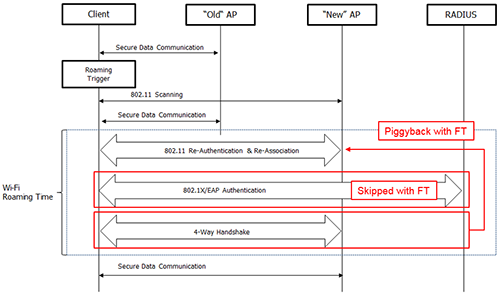
\includegraphics[scale=1.08]{80211r.png}

\subsubsection{802.11k Radio Resource Measurement}

A 802.11k, más néven Radio Resource Measurement (RRM) szabvány létrehozza a csatornák optimalizált listáját, ezzel segíti a közeli, roamingcélként szolgáló hozzáférési pontok gyors megkeresését. Amikor az aktuális hozzáférési pont jele gyengül, az eszköz további hozzáférési pontokat keres a listából, ezáltal elkerülve a teljes tartomány átvizsgálását.

% TODO: Nyelvi komplexitás csökkentése

A szabvány része a Beacon Report is, amely lehetővé teszi az STA számára, hogy lekérje önmaga számára a barangoláshoz ajánlott hozzáférési pontok listáját. Azonban ha ezek az információk helytelenek, akkor az állomás összezavarodhat. A legjobb eredmény elérése érdekében a beacon jelentésben az AP megkaphatja az állomástól a többi AP távolságát.

TODO: network packet capture image
. % https://support.apple.com/hu-hu/HT202628



\subsubsection{802.11v Wireless Network Management}

A 802.11v Wireless Network Management (WNM) szabvány célja, hogy lehetővé tegye a hálózati infrastruktúra és az STA-k közötti hatékony információcserét a teljes hálózat teljesítményének optimalizálása érdekében.

A szabvány legfontosabb funkciója a BSS Transition Management (BTM).

Általában az állomások nem tudják, hogy mi történik a hálózatban, és nem tudják, hogy melyik hozzáférési pont a legjobb választás. A BTM egy AP kérheti az állomástól, hogy váltson másik csatornára vagy hozzáférési pontra.

Azonban az állomás nem köteles elfogadni a kérést, és a BTM nem garantálja, hogy az állomás elfogadja a kérést. Az AP az Abridged Bit beállításával jelezheti, hogy erősen ajánlja a váltást.

A Disassociation Imminent Bit beállításával az AP jelezheti, hogy az állomásnak a disassociation timer-ben meghatározott másodpercen belül el kell hagynia a hálózatot.

TODO: BTM packet capture image


\subsection{Az OpenWrt hostapd és parancsai}

A \texttt{hostapd} egy hozzáférési pontokhoz és hitelesítési kiszolgálókhoz készült felhasználói tartományból elérhető szolgáltatás. \cite{hostapd}

OpenWrt rendszeren az ubus segítségével lehet legkönnyebben kommunikálni a hostapd-val.

Az \texttt{ubus} a projekt neve, amely egy daemonból, egy könyvtárból és egy parancssorból áll. Ezen kívül a \texttt{uhttpd-mod-ubus} modul segítségével a webes felületen keresztül is elérhetővé tehető. \cite{hostapd_config}

\begin{lstlisting}[language=Bash]
  Usage: ubus [<options>] <command> [arguments...]
  Options:
   -s <socket>:		Set the unix domain socket to connect to
   -t <timeout>:		Set the timeout (in seconds) for a command to complete
   -S:			Use simplified output (for scripts)
   -v:			More verbose output
   -m <type>:		(for monitor): include a specific message type
        (can be used more than once)
   -M <r|t>		(for monitor): only capture received or transmitted traffic

  Commands:
   - list [<path>]			List objects
   - call <path> <method> [<message>]	Call an object method
   - subscribe <path> [<path>...]	Subscribe to object(s) notifications
   - listen [<path>...]			Listen for events
   - send <type> [<message>]		Send an event
   - wait_for <object> [<object>...]	Wait for multiple objects to appear on ubus
   - monitor				Monitor ubus traffic
\end{lstlisting}

\subsubsection{A Wi-Fi kliensek listázása}

A BSS-hez csatlakozott kliensek listázásához a következő parancsot kell kiadni:

\begin{lstlisting}[language=Bash]
  root@OpenWrt:/ ubus call hostapd.$BSS get_clients
  {
    "freq": 5580,
    "clients": {
        "d8:f8:83:9d:52:dd": {
        "auth": true,
        "assoc": true,
        "authorized": true,
        "preauth": false,
        "wds": false,
        "wmm": true,
        "ht": true,
        "vht": true,
        "he": true,
        "wps": false,
        "mfp": false,
        "mbo": false,
        "rrm": [113, 0, 0, 0, 0],
        "extended_capabilities": [4, 0, 64, 0, 1, 0, 64, 64, 0, 0, 32],
        "aid": 3,
        "signature": "wifi4|probe:0,1,45,191,255,221(0050f2,8),htcap:19ef,htagg:17,htmcs:0000ffff,vhtcap:039071f6,vhtrxmcs:0000fffa,vhttxmcs:2000fffa|assoc:0,1,33,36,48,45,127,191,255,221(001735,8),70,59,221(0050f2,2),htcap:19ef,htagg:17,htmcs:0000ffff,vhtcap:039051f6,vhtrxmcs:0000fffa,vhttxmcs:2000fffa,txpow:1600,extcap:0400400001004040000020",
        "bytes": { "rx": 6035050799, "tx": 1296173698 },
        "airtime": { "rx": 17207474893, "tx": 15158693919 },
        "packets": { "rx": 4254865, "tx": 1606104 },
        "rate": { "rx": 240190000, "tx": 240190000 },
        "signal": -54,
        "capabilities": {
          "vht": {
            "su_beamformee": true,
            "mu_beamformee": true,
            "mcs_map": {
                "rx": {
                "1ss": 9, "2ss": 9, "3ss": -1, "4ss": -1, "5ss": -1, "6ss": -1, "7ss": -1, "8ss": -1
                },
                "tx": {
                "1ss": 9, "2ss": 9, "3ss": -1, "4ss": -1, "5ss": -1, "6ss": -1, "7ss": -1, "8ss": -1
                }
            }
          }
        }
      }
    }
  }
\end{lstlisting}

\subsubsection{A 802.11v transition request küldése}


\begin{lstlisting}[language=Bash]
  root@OpenWrt:/ ubus call hostapd.Mora_Network bss_transition_request '{"addr": "50:3D:C6:5B:81:E5", "reassoc_delay": 10, "disassociation_timer": 5, "validity_period": 30, "abridged": 1}' && sleep 5 && ubus call hostapd.Mora_Network del_client '{"addr" : "50:3D:C6:5B:81:E5", "deauth": true, "ban_time": 10000 }'
\end{lstlisting}


\begin{lstlisting}[language=Bash]
  root@OpenWrt:/ ubus call hostapd.Mora_Network bss_mgmt_enable '{ "neighbor_report": true, "beacon_report": true, "link_measurements": true, "bss_transition": true }'
\end{lstlisting}

\begin{lstlisting}[language=Bash]
  root@OpenWrt:/ ubus call hostapd.Mora_Network link_measurement_req '{ "addr": "FE:ED:AD:BE:EE" }'
\end{lstlisting}

% todo roaming, HT VHT, rrm_nr_get_own

\section{Terheléskiegyenlítés}

\section{Eredmények}

\subsection{Mérési környezet és metrikák}

\subsubsection{Prometheus}

\subsubsection{Grafana}

\subsubsection{A lokális tesztelés környezete}

\subsubsection{A kollégium hálózatán végzett mérések}




%laptörés:
\newpage

\section*{Függelék}
\subsection*{A program forráskódja}
A függelékbe kerülhetnek a hosszú táblázatok, vagy mondjuk egy programlista:
% \begin{lstlisting}[language=Python]
% for i in range(3):
% 	print(i)
% \end{lstlisting}


\section*{Nyilatkozat}
\noindent
Alulírott \@author, programtervező informatikus szakos hallgató, kijelentem, hogy a dolgozatomat a Szegedi Tudományegyetem, Informatikai Intézet XY Tanszékén készítettem, XY  diploma megszerzése érdekében.
%TODO tanszek es diplomahoz valami
Kijelentem, hogy a dolgozatot más szakon korábban nem védtem meg, saját munkám eredménye, és csak a hivatkozott forrásokat (szakirodalom, eszközök, stb.) használtam fel.

Tudomásul veszem, hogy szakdolgozatomat a Szegedi Tudományegyetem Diplomamunka Repozitóriumában tárolja.

\vspace*{2cm}

\begin{tabular}{lc}
Szeged, \today\
\hspace{2cm} & \makebox[6cm]{\dotfill} \\
& aláírás \\
\end{tabular}

\section*{Köszönetnyilvánítás}

Ezúton szeretnék köszönetet mondani \textbf{X. Y-nak} ezért és ezért \ldots

%\section*{hivatkozások}


\printbibliography

%\bibliography{hivatkozasok}{}
% \bibliographystyle{plain}
% \addcontentsline{toc}{section}{Hivatkozások}

\end{document}
